% !TEX encoding = UTF-8 Unicode
% !TEX root = ../thesis.tex
% !TEX spellcheck = en-US
%%=========================================



\chapter{Implementation}

% Hololens, UWP, WMR

\section{Requirements}

% cadavers difficult to get, vr -> less awareness
%
%


The first meeting initializing the project took place at VRLab Dragvoll in early September, here I was introduced to the general background and the problem description of how Witter and others envisioned the use of AR for neuroanatomical education. It was explained how cadavers for education are difficult to acquire and [\dots]. 
Another problem we discussed was related to the difference in medium between VR and AR. While the application \nameref{chap:vrvis} did have many of the features envisioned, and could have been a basis for further development. The fact that is was implemented in VR was problematic for the envisioned use cases. Being completely enclosed visually limits its use case in lectures and in any use case with collaboration in a physical space. Generally the loss of spatial awareness and eye contact as a result of using VR headsets was though of as an impediment for using VR for such an application. 
% something about the data set?
Thus, we had an outline of a neuroanatomical education tool in AR using the HoloLens 2 and concluded with some questions and requirements for the project:

\begin{enumerate}\label{mennoslist}
    \item Can the current VR dataset\footnotemark be used in the HoloLens 2 AR environment?
    \item If not, which steps need to be taken to use the segmented WHS rat brain to develop a suitable 3D model that can be used in AR?
    \item Develop an optimal user interface for a single person to explore the rat brain as if the user is doing a dissection of a real brain.
    \item Develop/test ways to make this a multiuser/shareable tool adequate in a teaching environment.
    \item Explore ways to integrate microscopical data into the AR representation.
    \item Describe/explore the feasibility to implement the system for Human neuroanatomy education.
\end{enumerate}

\footnotetext{Referring to \nameref{chap:vrvis}.}

Here items 1-4 were deemed critical for the project, while 5 and 6 were dependent on the progress made.

This meeting together with the list formed a clear problem description and can be seen as the initial discovery process of the project. Though the following period of exploring the newly arrived HoloLens 2 and its capabilities, we formed a set of \textit{system requirements}. 
System requirements are descriptions of how a system should operate, what it should be able to do and the constraints of its operation. The requirements must reflect the stakeholders needs for the system \citep{PUboka}. System requirements are generally split into functional requirements, which describe specifics of what the system (and its sub-systems) should do, and non-functional requirements, which generally are descriptions of the user experience of the system as a whole. 
What follows are the system requirements decided on for the application: 

\subsection*{Functional Requirements}
\begin{enumerate}
    \item {
        \textbf{Implement a brain dissection tool in AR.}\\
        The app should render a brain at sufficient quality for educational use, and have the tools for creating a dissection experience in AR.
        
    }
    \item {
        \textbf{The application must run in HoloLens 2 and at least one mobile platform}\\
        The ability to run a version for the app on multiple platforms is essential for the purpose of this project. While the main platforms are HoloLens and mobile, others may also be implemented in the future. 
    }

    \item {
        \textbf{Implement cross-platform collaboration over network}\\
        For the application to have value above a single user it is important that it can be used with a HoloLens and a more accessible platforms in a collaborative manner. 
    }


\end{enumerate}

\subsection*{Non-Functional Requirements}

\begin{enumerate}
    \item {
        \textbf{Medical students should find educational use for the app.}\\
        It is critical that there is educational value in the application. 
    }
    \item {
        \textbf{The application should be usable without outside guidance.}\\
        The app should have a clear and understandable design, such that a new user should be able to navigate the app by them self, even with minimal experience with AR.
    }
    \item {
        \textbf{All relevant usability criteria for a mixed reality app should be met.}\\
We should work to not fall under the 'meets' criteria on any relevant metric in the App quality criteria\footnote{https://docs.microsoft.com/en-us/windows/mixed-reality/develop/platform-capabilities-and-apis/app-quality-criteria}. This includes criteria on; FPS, spatial anchoring and view comfort. 
    }
\end{enumerate}

% and non-functional requirements, which describe  


\section{Software Process}
% https://www.wikipendium.no/TDT4140_Programvareutvikling/nb/#kapittel-2-software-processes

% Incremental development etc. \#agile
% \large{Where everything I learned in PU should shine!}

Even though I have developed the Nevrolens application by myself, I have strived to use best practices for a software development workflow. These practices have generally grown out of the the needs of a multi-developer setting, enabling simpler use of collaboration and version control. Though their value possibly increases exponentially by the number of team members, I have found value in the structure and clarity I find in the workflow. 

\begin{figure}[h]
    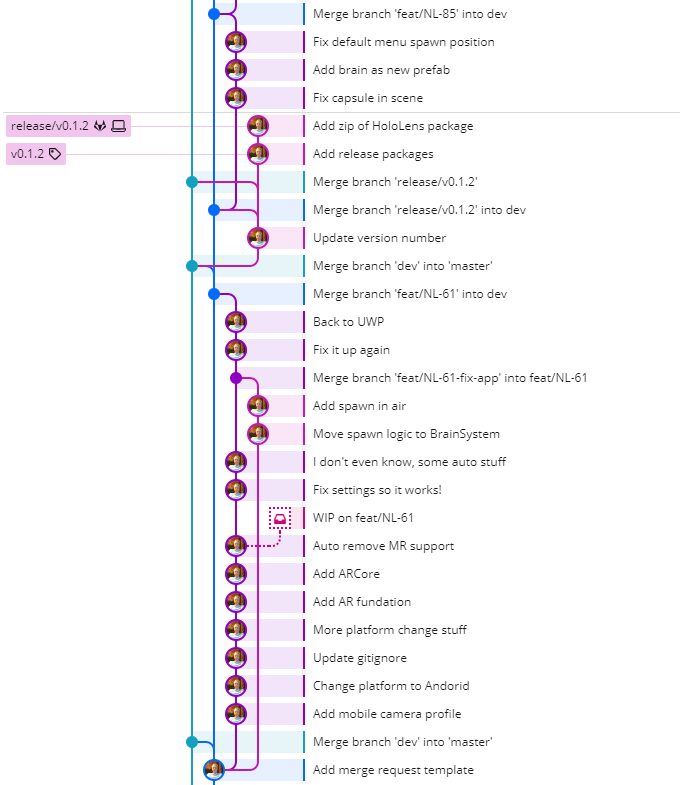
\includegraphics[width=0.33\textwidth]{fig/gitkraken_gitlog}
    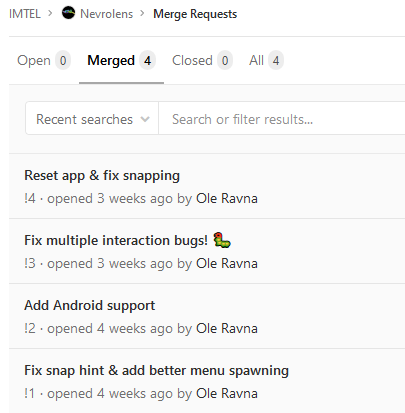
\includegraphics[width=0.33\textwidth]{fig/mergerequests}
    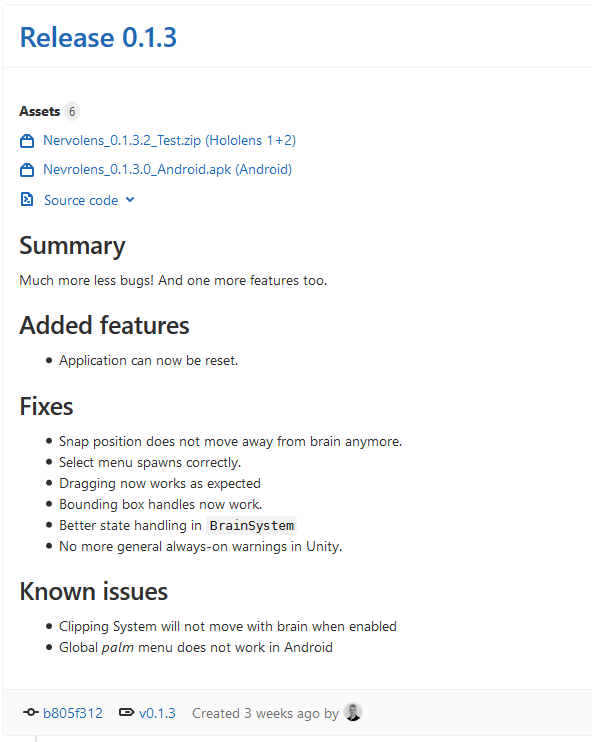
\includegraphics[width=0.33\textwidth]{fig/release_gitlab}
    \caption{Feature branches, merge requests and releases.}
\end{figure}

My workflow is based on \textit{Gitflow}, a workflow framework optimized for continuous software development. In short, this is just a very basic rule set for branch-naming and the sanctity of the master-branch (requiring merge requests of only product ready code), within the version control system \nameref{chap:git}. It does however act as a fundament which enables practices like rapid release cycles, because of the clearly define production ready state, and the integration with lean development technics like Kanban. This stems from the parallels between feature-branches in Gitflow and the \textit{ticket} in Kanban. In practice, this means that tickets, with issues or new features for the app, are created on in the \textit{Backlog} column of the Kanban board and are then moved to \textit{Doing} column simultaneously as a feature-branch is created with the ID of the ticket, e.g. \texttt{feat/NL-42}. All of this is automated in the Git management tool \nameref{chap:gitkraken}, which manages both the git-repo and the Kanban board.

\begin{figure}[h]
    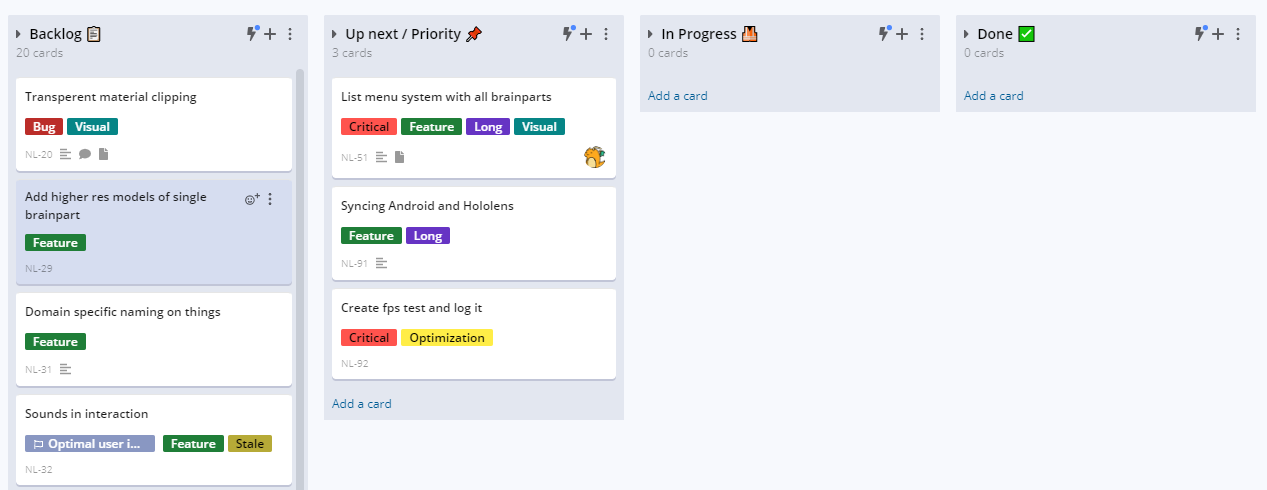
\includegraphics[width=\textwidth]{fig/kanban2}
    \caption{A snapshot of the Kanban board in GitKraken, after a development sprint, when completed tickets are archived (closed).\\ Note: \textit{Priority} acts as pined tickets on \textit{Backlog}, as the backlog tends to sizeable.}
    \label{fig:kanban}
\end{figure}

This workflow, by design, supports an agile development process. Agile approaches to software development are generally human-centered, valuing individuals and interactions over processes and tools\footnote{The Agile Manifesto https://agilemanifesto.org/}, and focused on iterating rather than upfront planning. This is ideas which are beneficial for single-developer or small teams especially when developing for new platforms like the HoloLens 2. 
While the project aims for an agile approach, the sprint cycle core to the agile development, where stakeholders are involved for regular feedback, has, due to a number of factors like COVID-19, only really been done for one cycle. However, the steps taken for an agile workflow should enable more agile development for the master project.

% One thing that I have not incorporated in to the workflow is user stories. The tickets in \autoref{fig:kanban} are written only for my understanding and will seem confusing and untidy for others. By using the concept of user stories 

% and will limited testing possibilities due to COVID-19 


% this enables me as a developer to test the product rapidly against users. 
% , this means having rules for branch naming, creating merge requests when merging to the `master`-branch, and 

\section{Development}

\subsection*{Rat brain model}
The rat brain model used in Nevrolens is, as of now, the same model as in \nameref{chap:vrvis} by \citet{Elden2017}. The original polygonal model created by Elden had a polygon count of around 16 million, he reduced this to around 3 million to run on a workstation computer with HTC Vive. The HoloLens 2 did not manage run smoothly with even that resolution, so I had to reduce it further to about 300,000 polygons.

\subsection*{Porting to Android}
The application was originally developed for HoloLens 2, but other platforms were always in mind and because of the use of \nameref{chap:mrtk}, deploying to other platform was relatively easy, within the documentation for MRTK, there was guides for how to build for Android. Interaction on Android is more complicated though. Because all interaction happens on screen additional effort has to be laid down to implement a good user experience on smartphone.  




